\documentclass{article}


\usepackage[english]{babel} % Language settings 
\usepackage{listings} % Schema Code settings

% Set page size and margins - Replace `letterpaper' with`a4paper' for UK/EU standard size
\usepackage[letterpaper,top=2cm,bottom=2cm,left=3cm,right=3cm,marginparwidth=1.75cm]{geometry}

% Useful packages
\usepackage{amsmath}
\usepackage{graphicx}
\usepackage[colorlinks=true, allcolors=blue]{hyperref}

\usepackage{float}

% title and author of the homework assignment 
\title{CSDS341 Project - Airline Querying System - Initial Report}
\author{Quynh Nguyen, Jiamu Zhang, Luke Zhang}

\begin{document}
	
	% set the underline style for schema code
	\lstset{
		language=C, 
		basicstyle=\ttfamily,
		moredelim=[is][\underbar]{-}{-}
	}
	
	\maketitle
	
	\section{Introduction}
	
	In recent decades, the growing demand for leisure and business travel leads to the prosperity of the airline market. An increasing number of people have been choosing to take flights to travel domestically or internationally. Therefore, an organized and comprehensive database that stores the airline system is critical for both travelers and crew to obtain plenty and simultaneous information.
	\\
	\\
	Although there do exist several flight databases or applications for commercial airlines, it is rare to find comprehensive information - including weather at the departure airport and destination, aircraft type, the total flight hour of pilots, and the number of luggage allowed - in just one database. This information offers travelers a chance to be better prepared for traveling.
	\\
	\\
	Since our airline querying system contains a relatively extensive data set, the crew members who choose to use our database are able to access the basic information about the travelers who will be on their flight and provides updates about the airline information. 
	
	\section{Entity-Relationship Model}
	
	\subsection{Assumptions}
	{Before performing the high-level design of the airline querying system, our group lists the following assumptions that need to be considered in our database systems.}
	
	\begin{enumerate}
		\item Assume that there have and only have two types of users of the airline querying system: travelers and crew.
		
		\item Assume that plane ticket information is stored in the database system and each ticket is only valid for one traveler. However, a traveler may own zero or more plane tickets. This matches the real situation in which travelers need to transfer their flights. 
		
		\item Assume that each ticket contains a specific seat location for exactly one flight. However, a flight may have multiple tickets being sold to travelers since a flight has obviously more than one seat.   
		
		\item Assume that a crew member can be either an air attendant or a pilot. Therefore, a crew member can serve zero or more flights. Additionally, a flight must be served by at least one crew. There does have a slight chance that a small propeller airplane only needs one crew member (i.e. the pilot).
		
		\item Assume that a flight is operated by exactly one areoplane. For example, figure 1 shows that the aircraft with registration number B-6075 is operating a specific flight (flight number: CA862) from Beijing(PEK) to Geneva(GVA). However, it is likely that one aeroplane can fly multiple flights. It is worth noticing that the  registration number is unique for each aeroplane.
		
		\item Assume that an aeroplane can only belong to one company. This database system does not consider private aeroplanes that do not belong to any company. For instance, the aeroplane B-6075 belongs to Air China. Additionally, a airline company can have multiple planes. 
		
		\item Assume that each airline company must have at least one airport as its hub, a place where the headquarter of the company locates and where the aeroplanes get maintenance and repaired. However, some large airports can provide services for multiple airline companies. For example, Los Angeles International Airport (LAX) is a hub for both United and Delta Airlines, and Delta Airlines has another hub : Detroit Metropolitan Airport (DTW).
		
		\item Assume that each flight can have multiple schedules, and a schedule can be mapped to multiple flights. It is common for most domestic flights to have the same flight flying the same route on two successive days. There is also a slight chance that two flights have the exact same schedule.
		
		\item Assume that each flight only departures from exactly one airport and only arrives at exactly one airport. However, an airport can have many flights. If a plane can arrive at two destinations simultaneously, then the pilot will win the next Nobel Physics Price.
		
		\begin{figure}[H]
			\centering
			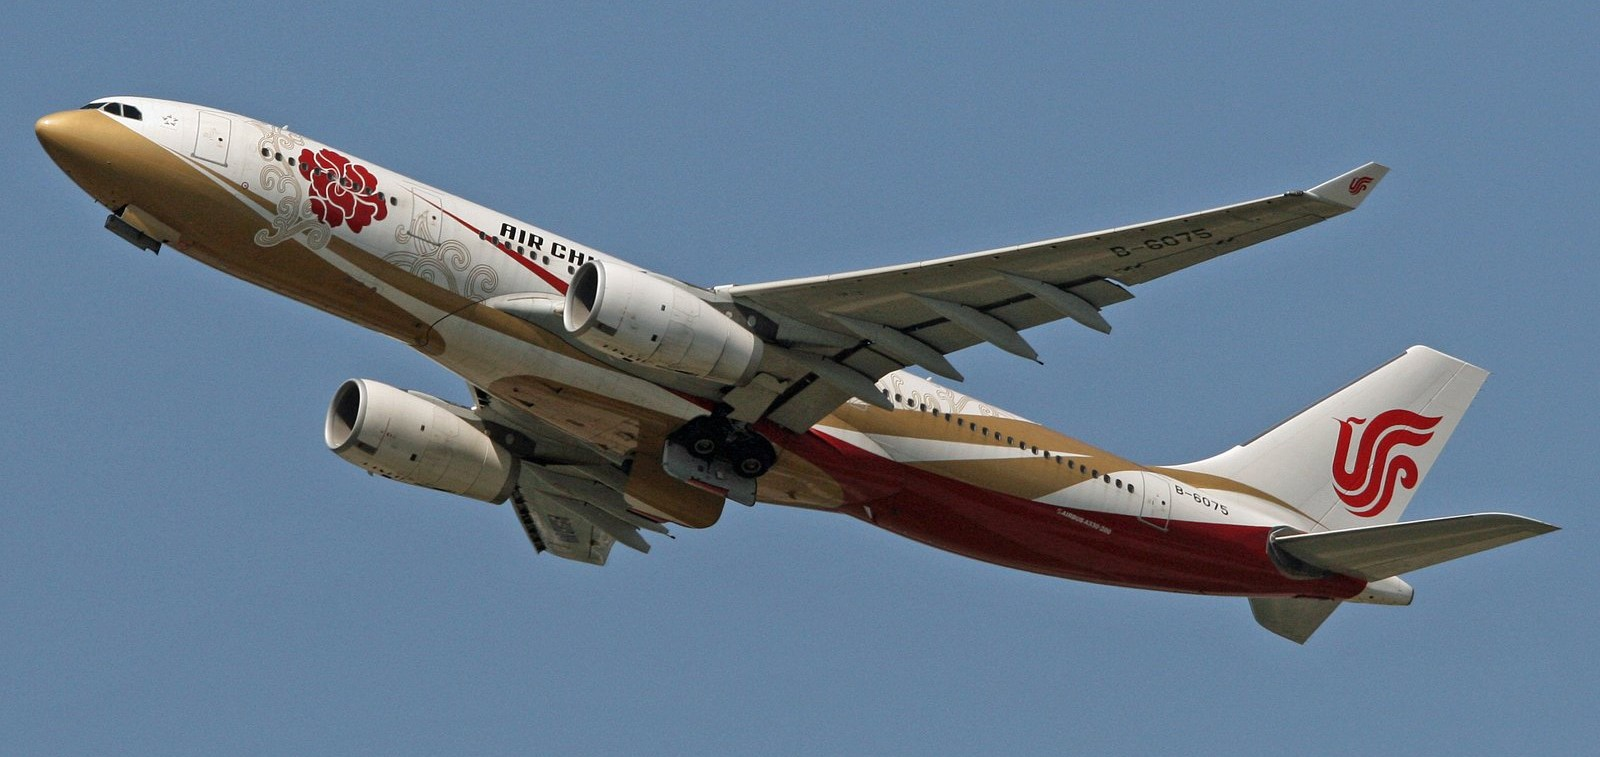
\includegraphics[width=100mm]{CSDS341_Project_B-6075.jpg}
			\caption{Aircraft with Registration Number B-6075 (\copyright Pascal Simon)}
		\end{figure}
		
	\end{enumerate}
	
	\subsection{ER Diagram}
	
	\begin{figure}[H]
		\centering
		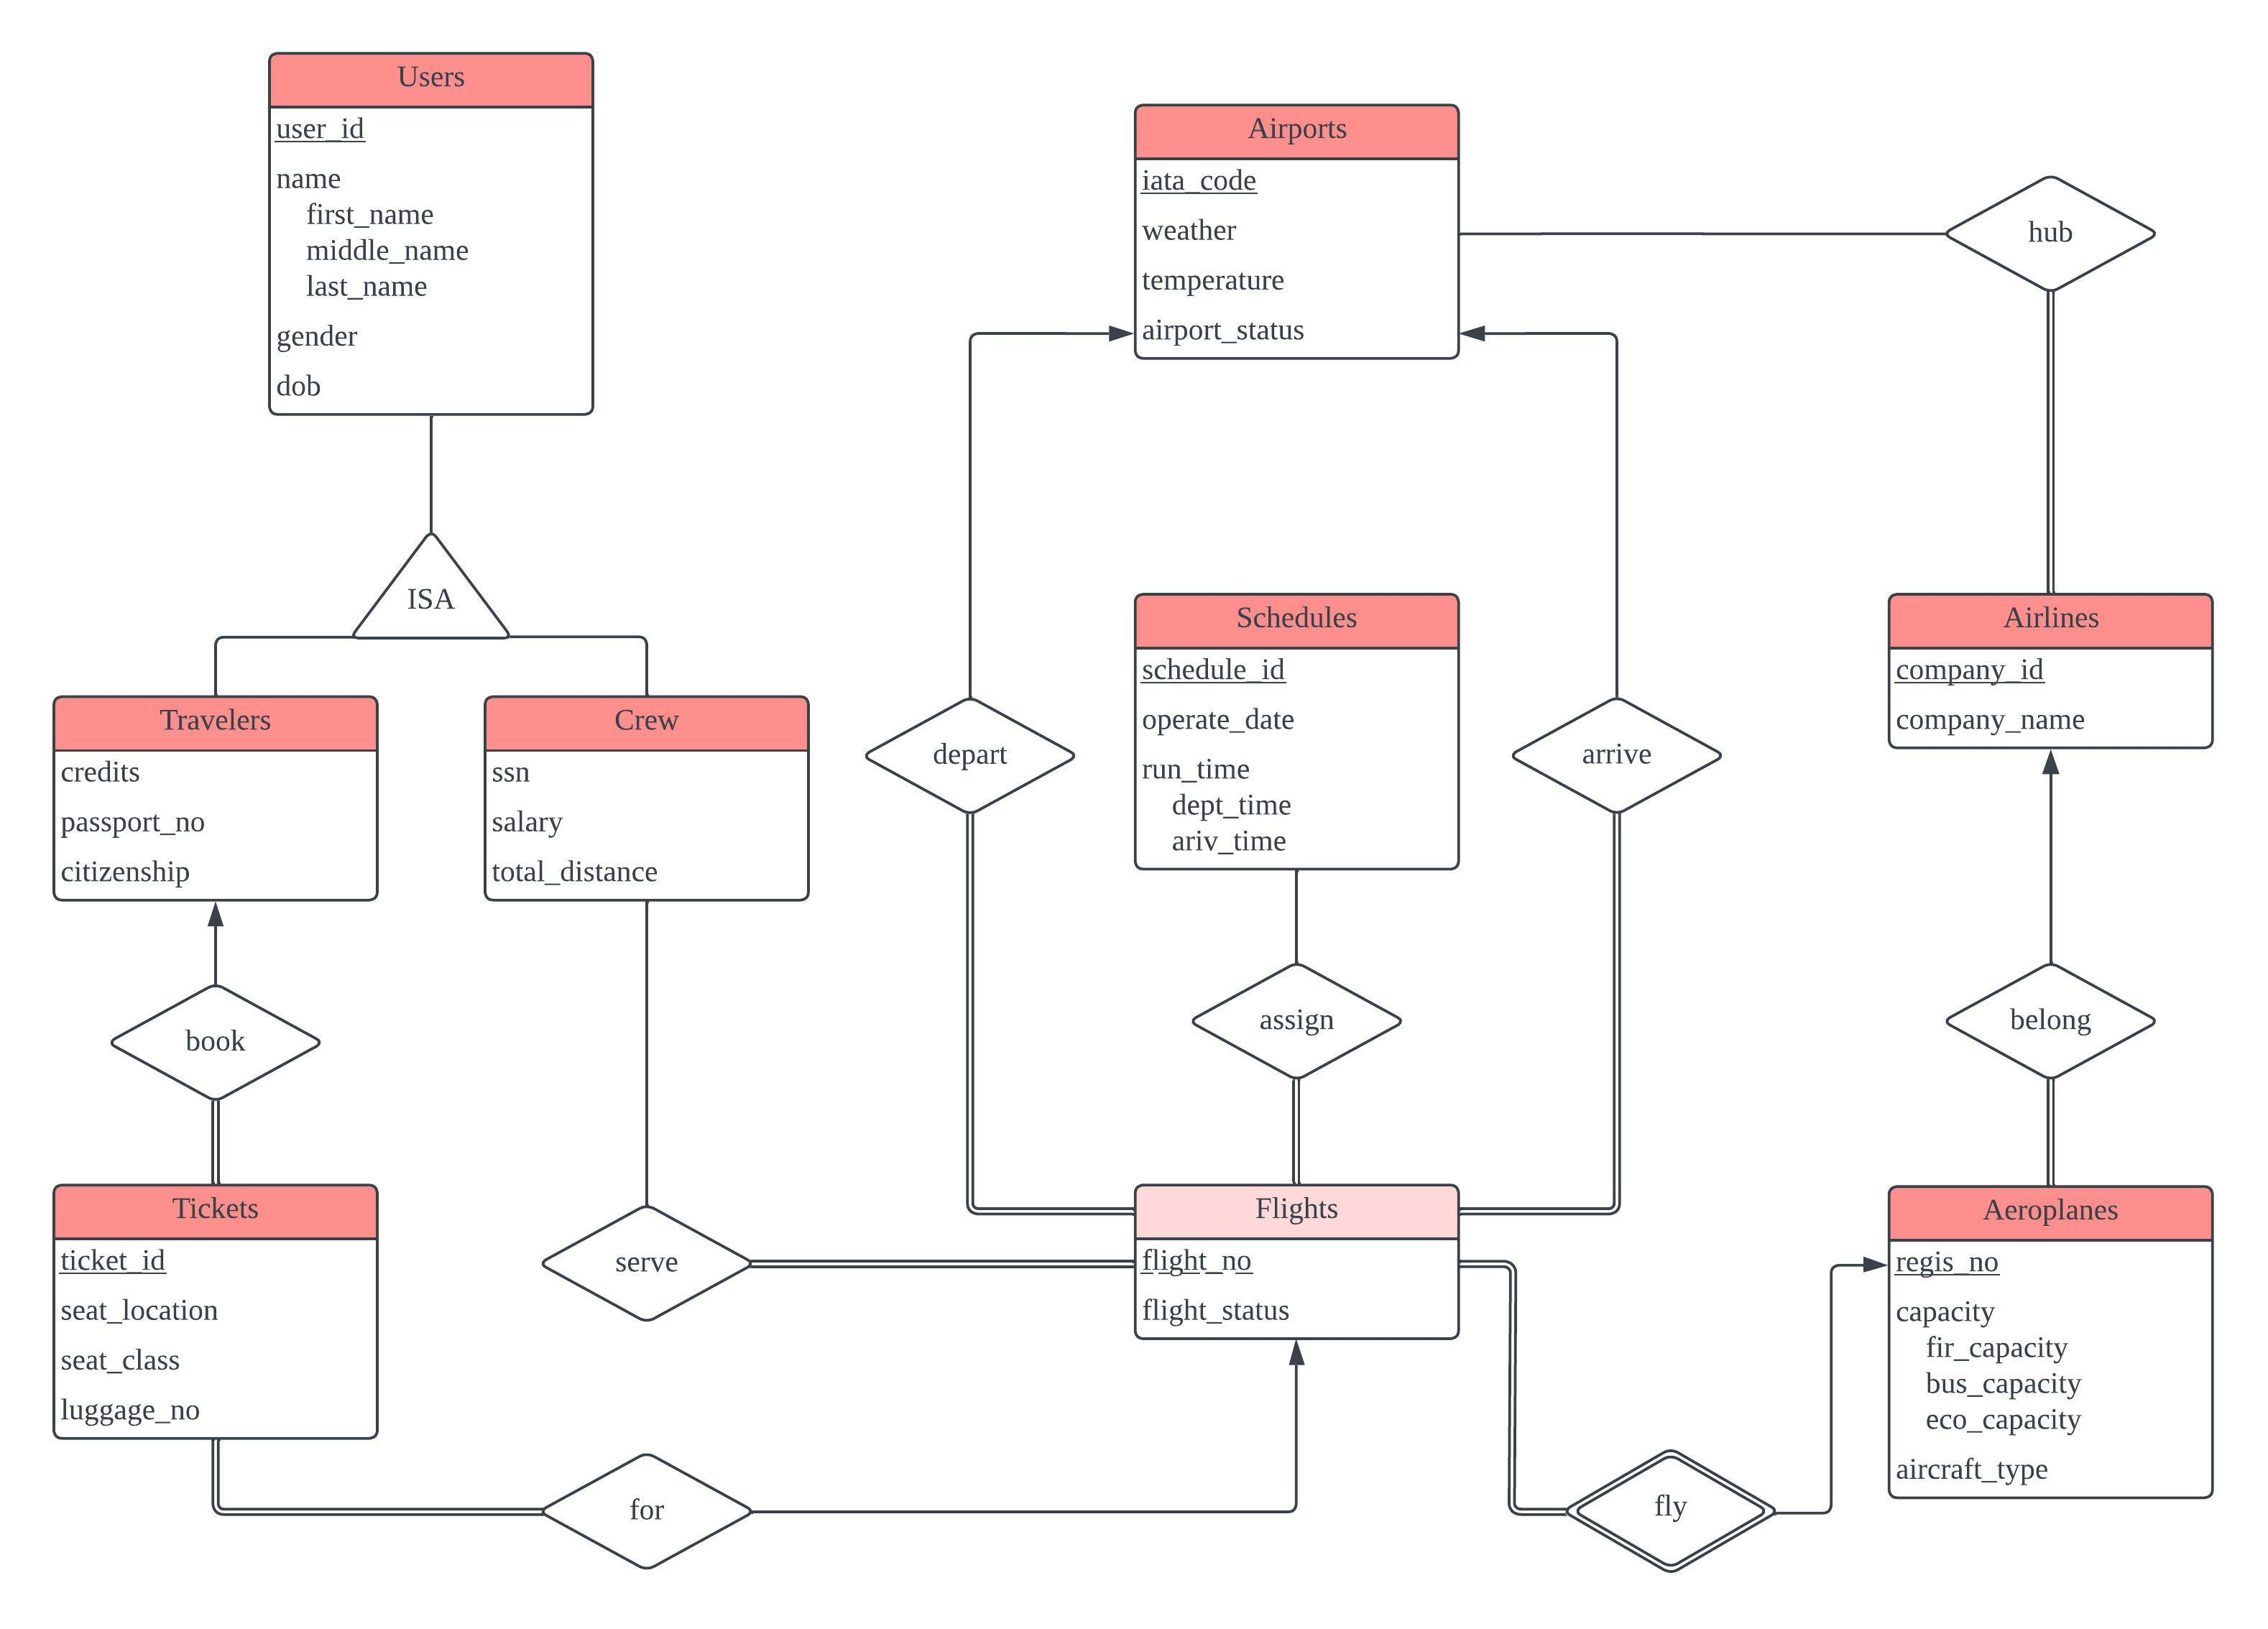
\includegraphics[width=140mm]{CSDS341_Project_ER_Diagram.jpeg}
		\caption{ER Diagram for Airline Querying System}
	\end{figure}
	
	\section{Schemas}
	
	\subsection{Strong Entities}
	\begin{lstlisting}[keepspaces=true]
Travelers(-user_id: int-,
          first_name: varchar(50),
          middle_name: varchar(50),
          last_name: varchar(50),
          gender: char(1),
          dob: date,
          credits: int,
          passport_no: varchar(20), 
          citizenship: varchar(30)
          )
	\end{lstlisting}    
	
	The entity \texttt{Travelers} is a type of \texttt{Users} in this Airline Querying Systems. The 
	\texttt{user\_id} attribute is the primary key of this entity.
	
	\begin{lstlisting}[keepspaces=true]
Crew(-user_id: int-,
     first_name: varchar(50),
     middle_name: varchar(50),
     last_name: varchar(50),
     gender: char(1),
     dob: date,
     ssn: int, 
     salary: double, 
     total_distance: int
     )
	\end{lstlisting}    
	
	The entity \texttt{Crew} is the other type of \texttt{Users} in this Airline Querying Systems. The 
	\texttt{user\_id} attribute is the primary key of this entity.
	
	\begin{lstlisting}[keepspaces=true]
Airports(-iata_code: char(3)-, 
         weather: varchar(15),
         temperature: int,
         airport_status: varchar(10)
         )
	\end{lstlisting}    
	
	The entity \texttt{Airports} stores the information of airports, with a primary key \texttt{iata\_code}. IATA Code stands for International Air Transport Association Code. It is a three-character code that is unique for each airport. For example, the IATA Code for Los Angeles International Airport is LAX.
	
	\begin{lstlisting}[keepspaces=true]             
Airlines(-company_id: int-,
         company_name: varchar(30)
         )
	\end{lstlisting}    
	
	The entity \texttt{Airports} stores the information of airports, with a primary key \texttt{iata\_code}. IATA Code stands for International Air Transport Association Code. It is a three-character code that is unique for each airport. For example, the IATA Code for Los Angeles International Airport is LAX.
	
	\begin{lstlisting}[keepspaces=true]               
Aeroplanes(-regis_no: varchar(10)-,
           fir_capacity: int,
           bus_capacity: int, 
           eco_capacity: int,
           aircraft_type: varchar(10)
           )
	\end{lstlisting}    
	
	The entity \texttt{Aeroplanes} stores the information of each aircraft, with a primary key \texttt{regis\_no} (registration number). Before each plane starts operating, it will be assigned a unique registration number.
	
	\begin{lstlisting}[keepspaces=true] 
Schedules(-schedule_id: int-, 
          operate_date: date,
          dept_time: time,
          ariv_time: time
          )
	\end{lstlisting}
	
	The entity \texttt{Schedules} stores the flight schedules. The primary key is \texttt{schedule\_id}.
	
	\subsection{Weak Entities}
	
	\begin{lstlisting}[keepspaces=true]
Tickets(-traveler_id: int-, 
        -order_no: int-, 
        seat_location: char(3),
        seat_type: char(1),
        luggage_no: int
        )
        Foreign Key (traveler_id) references (Travelers.user_id)
	\end{lstlisting}    

	The weak entity \texttt{Tickets} stores the ticket information of each traveler. The primary key of the weak entity is \texttt{traveler\_id} and \texttt{order\_no}. 

	\begin{lstlisting}[keepspaces=true]        
		
Flights(-regis_no: int-, 
        -flight_no: varchar(7)-,
        flight_status: varchar(10)
        )
        Foreign Key (regis_no) references (Aeroplanes.regis_no)
	\end{lstlisting}

	The weak entity \texttt{Flights} stores the information of each flight operated by each aeroplane. The primary key of the weak entity is \texttt{regis\_no} and \texttt{flight\_no}.

	\subsection{Relationships}
	
	\begin{lstlisting}[keepspaces=true]
for(-traveler_id: int-, 
    -order_no: int-,
    regis_no: int, 
    flight_no: varchar(7)
    )
    Foreign Key (traveler_id) references (Travelers.user_id)
    Foreign Key (order_no) references (Tickets.order_no)
    Foreign Key (regis_no) references (Aeroplanes.regis_no)
    Foreign Key (flight_no) references (Flights.flight_no)
	\end{lstlisting}    

	The \texttt{for} relationship stores the information regrading tickets for flights. Since each ticket is for exactly one flight and a flight can have many tickets, this is a many-to-one relationship. Therefore, the primary key from the many side (i.e. \texttt{Tickets.order\_no} and \texttt{Travelers.user\_id}) should be set as the primary key of this relationship.

	\begin{lstlisting}[keepspaces=true]        
serve(-crew_id: int-, 
      -regis_no: int-, 
      -flight_no: varchar(7)-
      )
      Foreign Key (crew_id) references (Crew.user_id)
      Foreign Key (regis_no) references (Aeroplanes.regis_no)
      Foreign Key (flight_no) references (Flights.flight_no)
	\end{lstlisting}    

	The \texttt{serve} relationship stores the information regarding how crew members serve for flights. Since each crew member can serve multiple flights and a flight may need multiple crews, this is a many-to-many relationship. Therefore, the primary key from both sides should be set as the primary key of this relationship.

	\begin{lstlisting}[keepspaces=true] 
depart(-regis_no: varchar(10)-,
       -flight_no: varchar(7)-,
       dept_iata_code: cahr(3)
       )  
       Foreign Key (regis_no) references (Aeroplanes.regis_no)
       Foreign Key (flight_no) references (Flights.flight_no)
       Foreign Key (dept_iata_code) references (Airports.iata_code)
	\end{lstlisting}    

	The \texttt{depart} relationship stores the information regarding departure information. Since each flight can depart from only one airport while an airport can have many departing planes, this is a one-to-many relationship. Therefore, the primary key from many sides (i.e. \texttt{Aeroplanes.regis\_no} and \texttt{Flights.flight\_no}) should be set as the primary key of this relationship.

	\begin{lstlisting}[keepspaces=true]
arrive(-regis_no: varchar(10)-,
       -flight_no: varchar(7)-, 
       ariv_iata_code: char(3),
       )  
       Foreign Key (regis_no) references (Aeroplanes.regis_no)
       Foreign Key (flight_no) references (Flights.flight_no)
       Foreign Key (ariv_iata_code) references (Airports.iata_code)
	\end{lstlisting}    

	The \texttt{arrive} relationship stores the information regarding arrival information. Since each flight can arrive only one airport while an airport can have many departing planes, this is a one-to-many relationship. Therefore, the primary key from many sides (i.e. \texttt{Aeroplanes.regis\_no} and \texttt{Flights.flight\_no}) should be set as the primary key of this relationship.

	\begin{lstlisting}[keepspaces=true]		
assign(-regis_no: varchar(10)-,
       -flight_no: varchar(7)-,
       -schedule_id: int-
       )
       Foreign Key (regis_no) references (Aeroplanes.regis_no)
       Foreign Key (flight_no) references (Flights.flight_no)
       Foreign Key (schedule_id) references (Schedules.schedule_id)
	\end{lstlisting}    

	The \texttt{assign} relationship stores the information regarding the mapping between flights and schedules. Since this is a many-to-many relationship, the primary key from both sides should be set as the primary key of this relationship.

	\begin{lstlisting}[keepspaces=true]	
hub(-company_id: int-,
    -iata_code: char(3)-
    )
    Foreign Key (company_id) references (Airlines.company_id)
    Foreign Key (iata_code) references (Airports.iata_code)
	\end{lstlisting}    

	The \texttt{hub} relationship stores the information regarding airline companies and their hub airports. Since this is a many-to-many relationship, the primary key from both sides should be set as the primary key of this relationship.

	\begin{lstlisting}[keepspaces=true]	
belong(-regis_no: varchar(10)-,
       company_id: int
       )
       Foreign Key (regis_no) references (Aeroplanes.regis_no)
       Foreign Key (company_id) references (Airlines.company_id)
	\end{lstlisting}

	The \texttt{belong} relationship stores the information regarding airline companies and planes they owned. Since this is a one-to-many relationship, the primary key from the many side (i.e. \texttt{Aeroplanes.regis\_no}) should be set as the primary key of this relationship.
	
	\subsection{Identifying Relationships}
	All the identifying relationships in the schema are merged with the weak entity. There is no need to create separate tables because that may cause redundancies.
	
\end{document}